\documentclass[11pt]{article}
\usepackage[margin=1in]{geometry}
\usepackage{booktabs}
\usepackage{graphicx}
\usepackage{caption}
\usepackage{xcolor}

\title{Original and Reproduced PIE-Bench Results}
\date{}

\begin{document}
\maketitle

\begin{figure}[htbp]
  \centering
  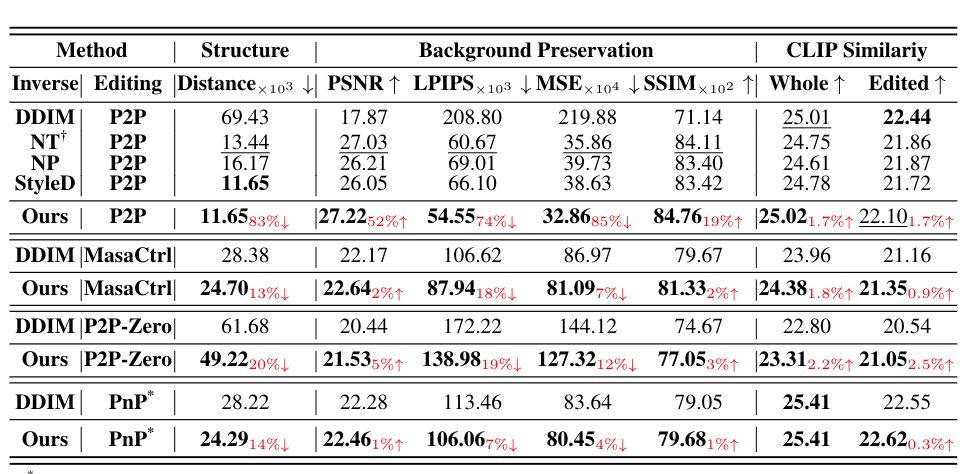
\includegraphics[width=\linewidth]{pnp_inversion_results.png}
  \caption{Original results supplied in \texttt{reports/pnp\_inversion\_results.png}.}
  \label{fig:original-results}
\end{figure}

\clearpage
\begin{table*}[htbp]
  \centering
  \small
  \caption{Original paper results and reproduced runs, paired by editor and inversion method. Structure distance and LPIPS are scaled by $10^3$, MSE by $10^4$, and SSIM by $10^2$. Reproduced values are PIE-Bench means rounded to two decimal places. Bold indicates the better value according to each metric direction; red flags a reproduced value whose absolute gap from the original exceeds 1.}
  \label{tab:original-reproduction-comparison}
  \resizebox{\textwidth}{!}{%
  \begin{tabular}{lllrrrrrrr}
    \toprule
    Editor & Inversion & Source & Structure ($\times 10^3$) $\downarrow$ & PSNR (dB) $\uparrow$ & LPIPS ($\times 10^3$) $\downarrow$ & MSE ($\times 10^4$) $\downarrow$ & SSIM ($\times 10^2$) $\uparrow$ & CLIP whole $\uparrow$ & CLIP edited $\uparrow$ \\
    \midrule
    P2P & DDIM & Original & \textbf{69.43} & 17.87 & 208.80 & 219.88 & 71.14 & 25.01 & 22.44 \\
    P2P & DDIM & Reproduced & \textcolor{red}{70.48} & \textbf{17.87} & \textbf{208.79} & \textbf{219.41} & \textbf{71.65} & \textbf{25.27} & \textbf{22.55} \\
    P2P & Direct Inversion & Original & \textbf{11.65} & \textbf{27.22} & \textbf{54.55} & \textbf{32.86} & \textbf{84.76} & 25.02 & 22.10 \\
    P2P & Direct Inversion & Reproduced & \textcolor{red}{31.55} & \textcolor{red}{22.53} & \textcolor{red}{126.55} & \textcolor{red}{92.38} & \textcolor{red}{78.49} & \textbf{25.21} & \textbf{22.31} \\
    \midrule
    MasaCtrl & DDIM & Original & 28.38 & 22.17 & 106.62 & 86.97 & 79.67 & 23.96 & 21.16 \\
    MasaCtrl & DDIM & Reproduced & \textcolor{red}{\textbf{27.09}} & \textbf{22.19} & \textcolor{red}{\textbf{105.34}} & \textbf{86.35} & \textbf{80.32} & \textbf{24.23} & \textbf{21.20} \\
    MasaCtrl & Direct Inversion & Original & 24.70 & 22.64 & 87.94 & 81.09 & 81.33 & 24.38 & 21.35 \\
    MasaCtrl & Direct Inversion & Reproduced & \textcolor{red}{\textbf{23.70}} & \textbf{22.67} & \textbf{87.85} & \textbf{80.85} & \textbf{81.85} & \textbf{24.60} & \textbf{21.46} \\
    \midrule
    P2P-Zero & DDIM & Original & 61.68 & 20.44 & \textbf{172.22} & 144.12 & 74.67 & 22.80 & 20.54 \\
    P2P-Zero & DDIM & Reproduced & \textbf{61.25} & \textbf{20.47} & 172.26 & \textbf{143.71} & \textbf{75.39} & \textbf{22.93} & \textbf{20.74} \\
    P2P-Zero & Direct Inversion & Original & 49.22 & 21.53 & 138.98 & \textbf{127.32} & 77.05 & 23.31 & 21.05 \\
    P2P-Zero & Direct Inversion & Reproduced & \textbf{49.09} & \textbf{21.57} & \textbf{138.39} & \textcolor{red}{129.77} & \textbf{77.73} & \textbf{23.47} & \textbf{21.08} \\
    \midrule
    PnP & DDIM & Original & 28.22 & 22.28 & 113.46 & 83.64 & 79.05 & 25.41 & 22.55 \\
    PnP & DDIM & Reproduced & \textbf{27.33} & \textbf{22.32} & \textbf{112.73} & \textbf{82.94} & \textbf{79.58} & \textbf{25.58} & \textbf{22.57} \\
    PnP & Direct Inversion & Original & 24.29 & 22.46 & 106.06 & 80.45 & 79.68 & 25.41 & 22.62 \\
    PnP & Direct Inversion & Reproduced & \textbf{23.35} & \textbf{22.46} & \textbf{105.49} & \textbf{79.93} & \textbf{80.22} & \textbf{25.64} & \textbf{22.67} \\
    \bottomrule
  \end{tabular}
  }
\end{table*}

\noindent All reproduced runs have metric summaries.

\end{document}
